\section{Diagramas de secuencia del sistema}
\label{sec:diagramas_secuencia}

    Los diagramas de secuencia UML 2.5 detallan la dimensión temporal y el intercambio cronológico de mensajes entre componentes: el cliente en React, los controladores REST, los servicios de aplicación en Spring Boot, los publicadores de eventos de dominio, la base de datos PostgreSQL y los servicios externos conectados.

    La plataforma implementa ochenta y seis casos de uso, pero la mayoría realiza operaciones estándar de lectura o actualización. Se seleccionaron diez escenarios con lógica distribuida, salvaguardas de concurrencia o sincronización asíncrona:

\begin{enumerate}
\item Recuperación segura de contraseña con doble fase y mitigación de enumeración.
\item Alta de inmueble base con geocodificación cartográfica y compensación transaccional.
\item Solicitud de reserva con validación temporal de calendario y notificación multicanal.
\item Transición de estados y formalización del cobro de fianza en reserva aceptada.
\item Adhesión a un espacio de convivencia mediante código efímero y asignación de membresía.
\item Registro de gasto compartido con cálculo de matriz contable y simplificación de balances.
\item Baja o expulsión de un miembro con validación de saldo cero y rebalanceo de tareas.
\item Planificación periódica de tareas domésticas y resolución de rescate gamificado.
\item Interacción con el asistente inteligente mediante ticket efímero y protocolo MCP.
\item Tramitación y resolución de denuncias con auditoría de chat y suspensión cautelar.
\end{enumerate}

    La recuperación de credenciales opera en dos fases desacopladas (figura \ref{fig:seq_recuperacion_contrasena}).

\begin{figure}[H]
    \centering
    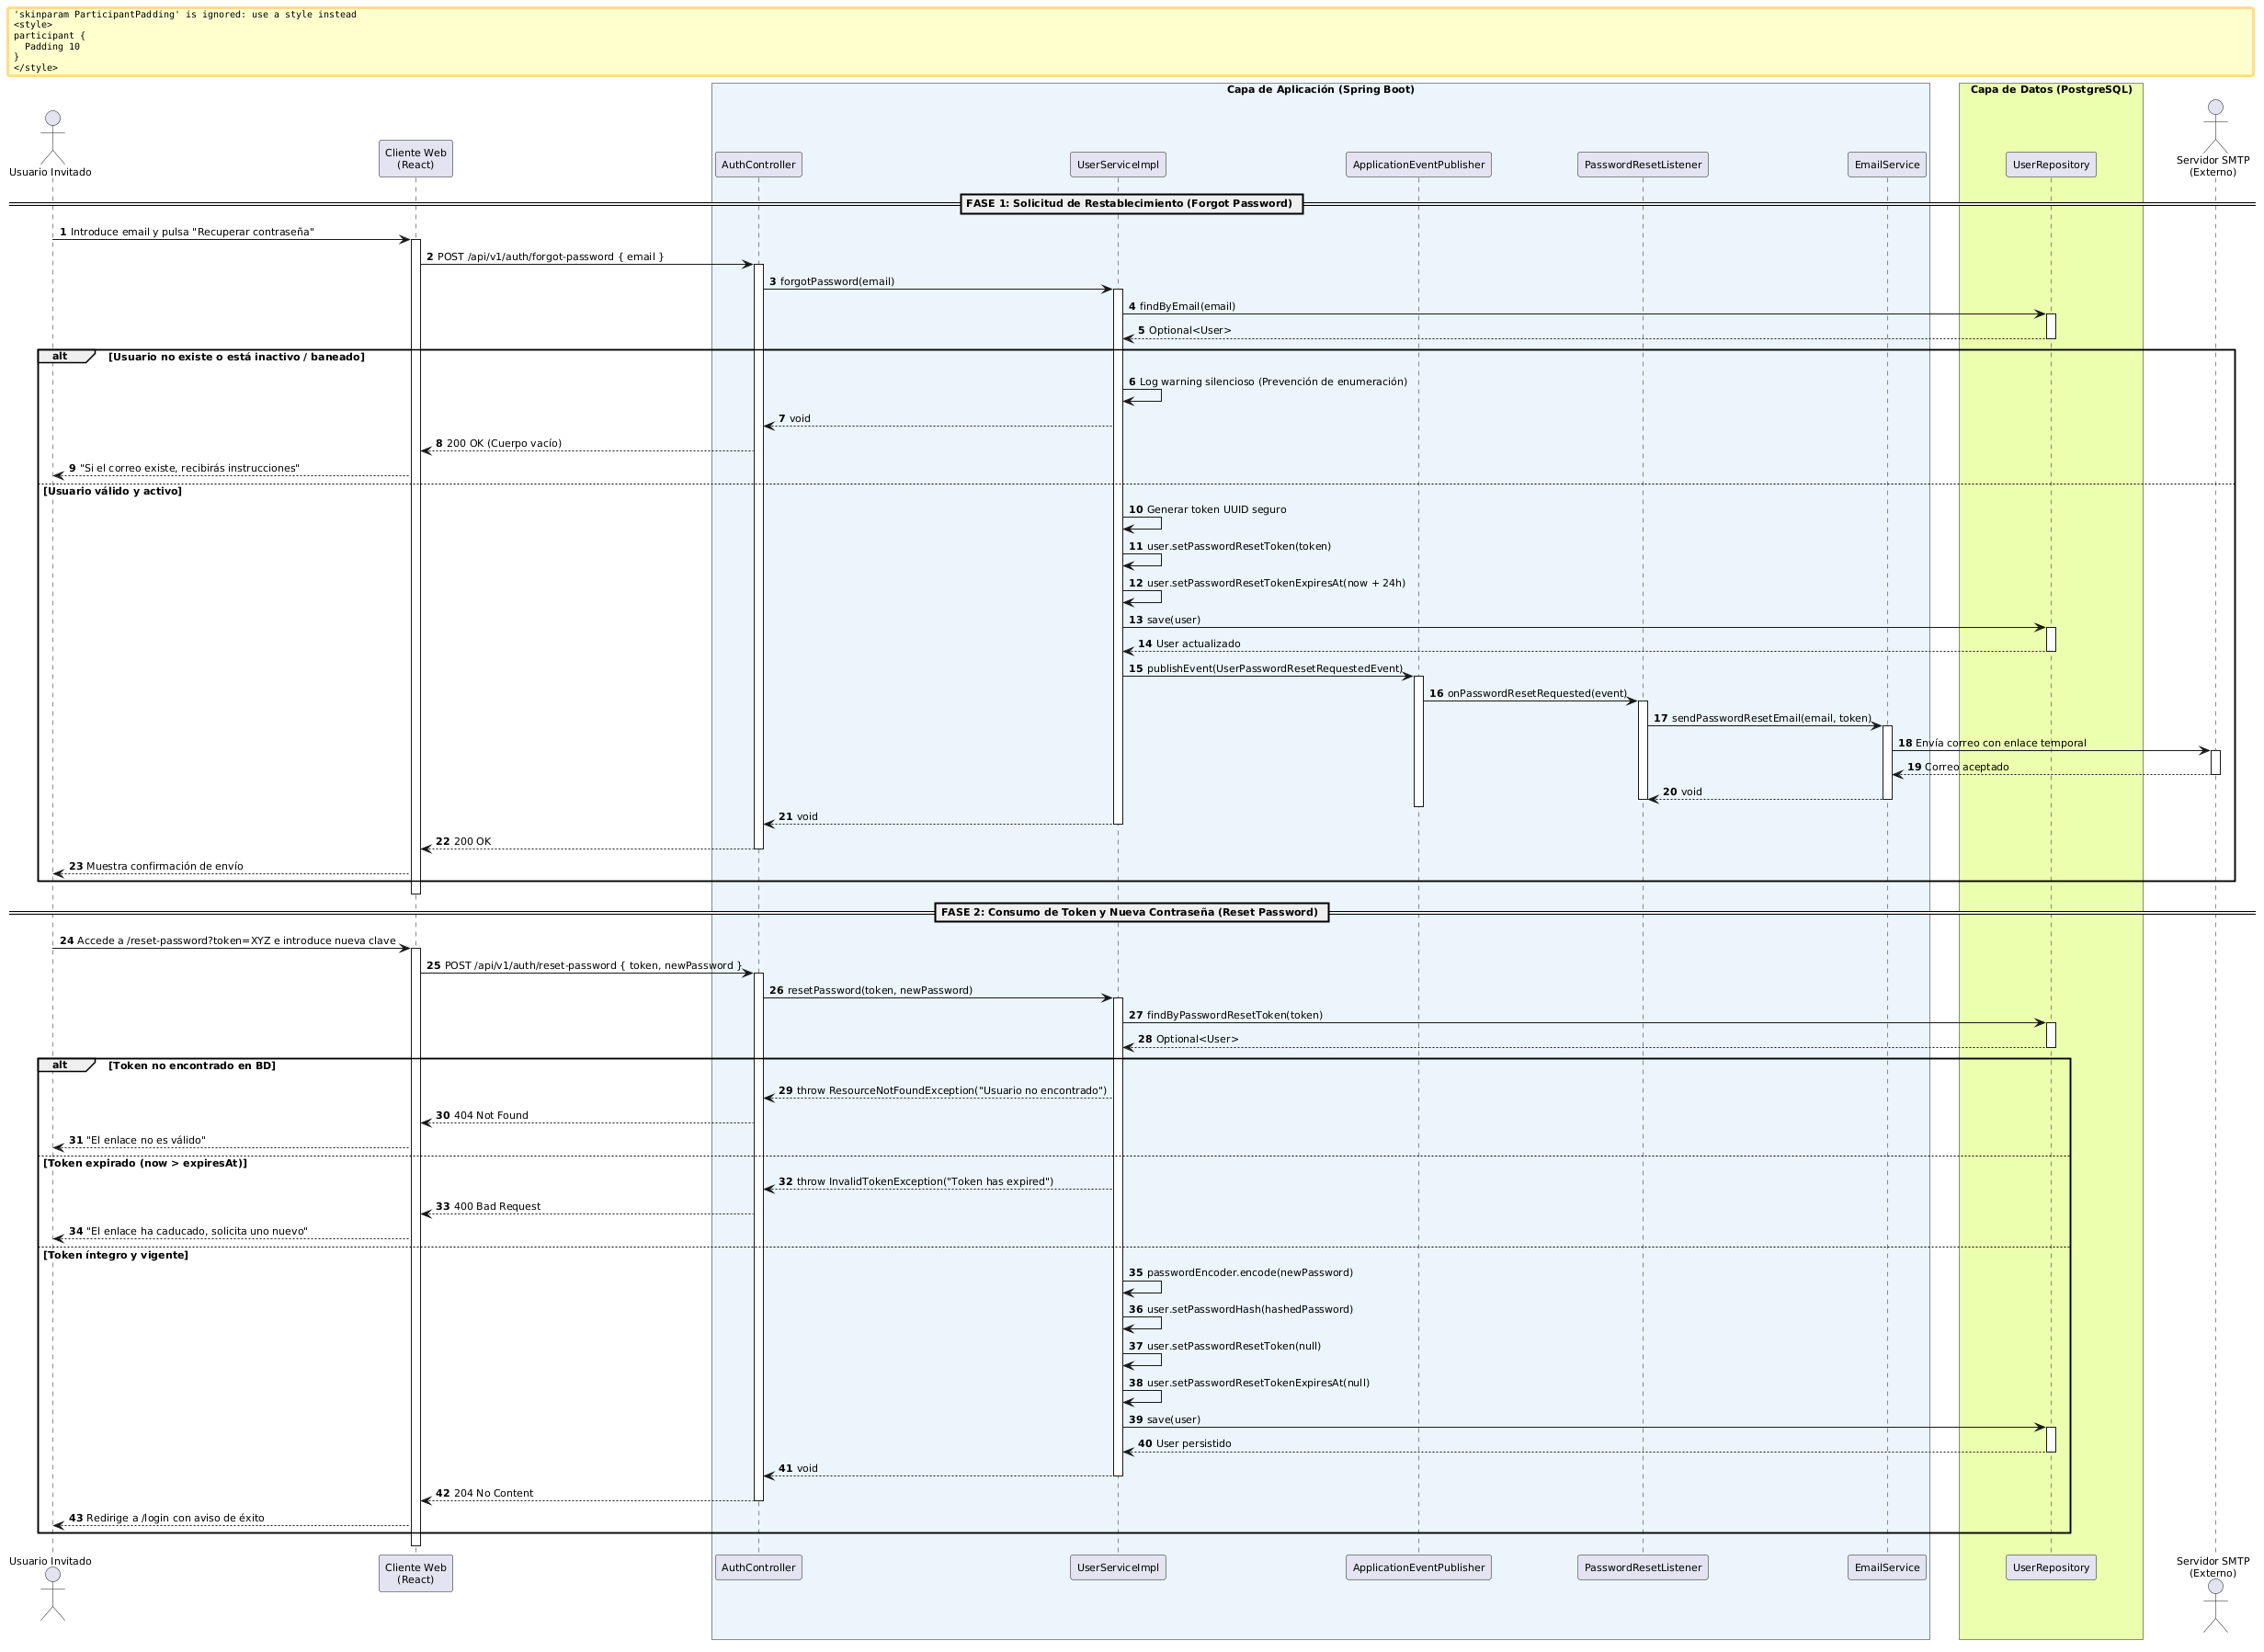
\includegraphics[width=0.95\textwidth]{AnalisisFuncional/img/seq_recuperacion_contrasena.png}
    \caption{Diagrama de secuencia del proceso de recuperación segura de contraseña}
    \label{fig:seq_recuperacion_contrasena}
\end{figure}

    El usuario introduce su correo electrónico en el formulario web. El sistema aplica una política de defensa contra ataques de enumeración de cuentas (\emph{Anti User-Enumeration}): si la dirección no existe en la base de datos o la cuenta está suspendida, el servicio genera una traza interna y retorna un código HTTP 200 con cuerpo vacío. La interfaz muestra un mensaje estándar de confirmación. Ningún atacante puede inferir qué cuentas están dadas de alta. Si la cuenta existe, se genera un identificador UUID temporal con 24 horas de validez y se persiste en base de datos. \texttt{ApplicationEventPublisher} dispara de inmediato la notificación en segundo plano para que el servicio de correo despache el mensaje sin bloquear la respuesta HTTP al cliente.

    El restablecimiento concluye cuando el usuario abre el enlace con el token temporal e introduce la nueva contraseña. El backend comprueba la existencia del token y verifica que no haya vencido la marca de tiempo. Si la validación es correcta, la clave se procesa con el algoritmo de dispersión (\emph{hashing}) con sal criptográfica, se invalida el token temporal y se persiste la entidad, retornando un código 204 que redirige al usuario hacia el formulario de inicio de sesión.

    El alta de propiedades físicas combina geocodificación cartográfica con almacenamiento multimedia (figura \ref{fig:seq_alta_inmueble}).

\begin{figure}[H]
    \centering
    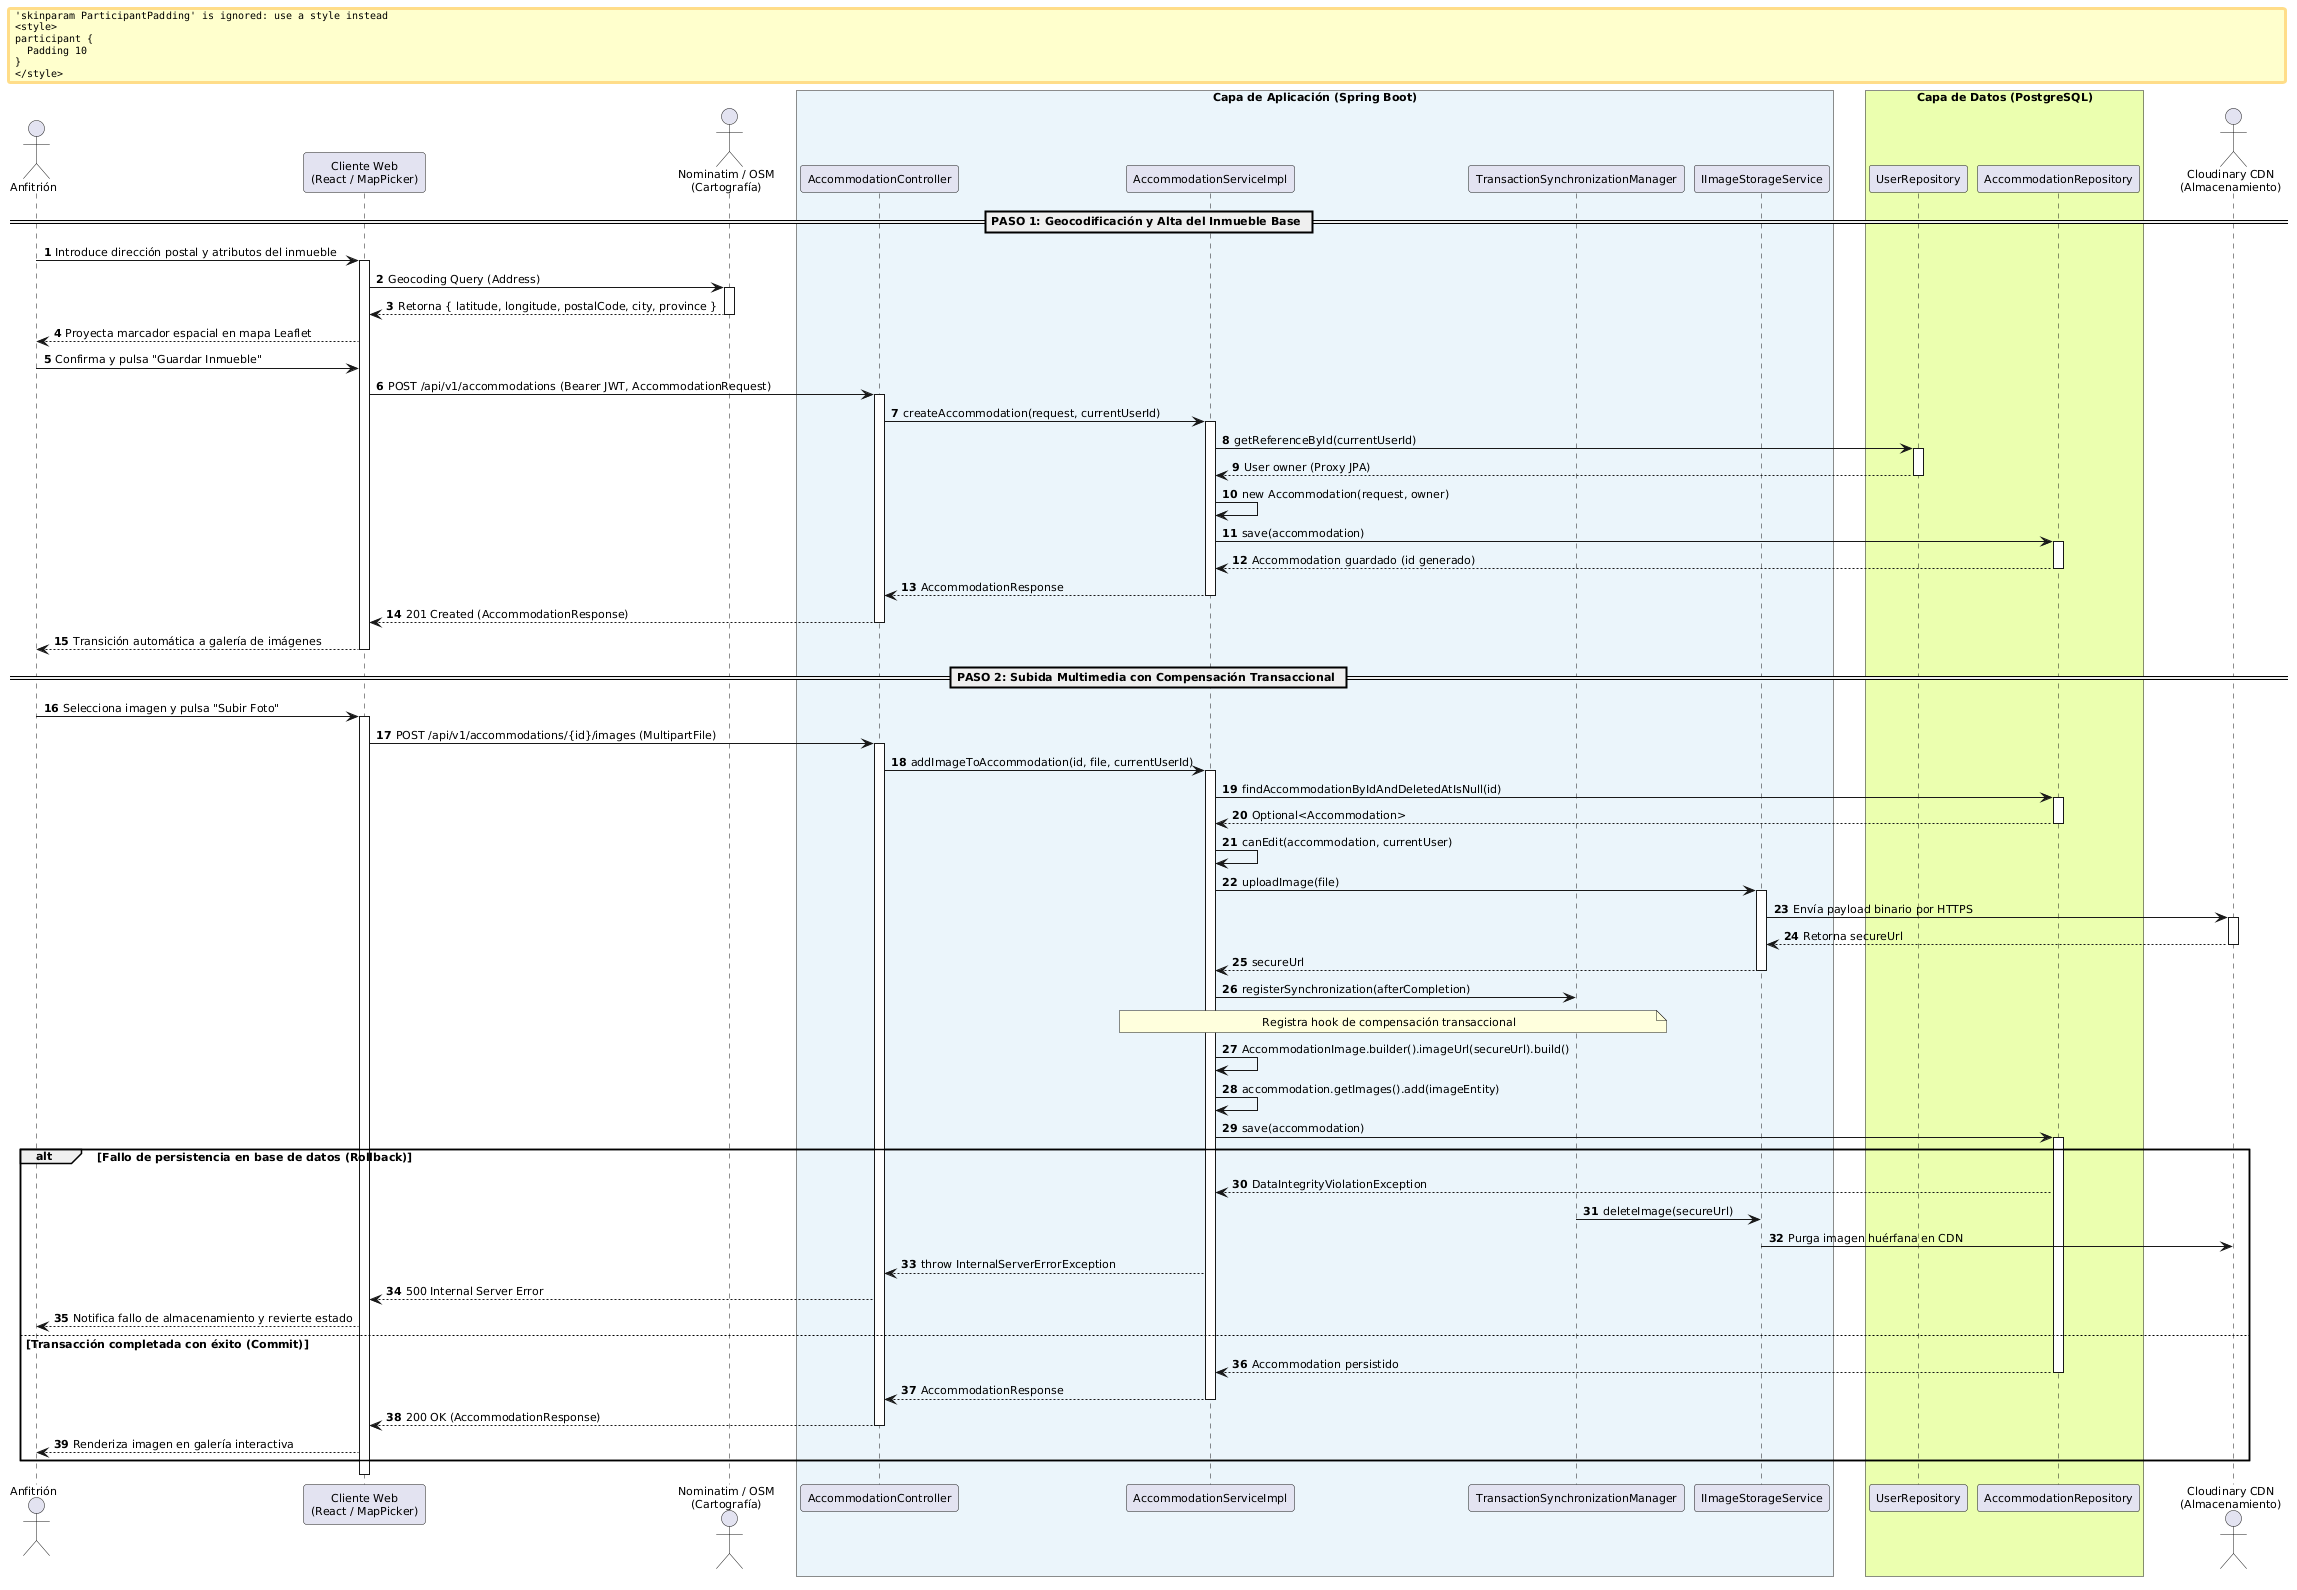
\includegraphics[width=0.95\textwidth]{AnalisisFuncional/img/seq_alta_inmueble.png}
    \caption{Diagrama de secuencia del alta de inmueble con geocodificación y compensación transaccional}
    \label{fig:seq_alta_inmueble}
\end{figure}

    El proceso se divide en dos fases. El anfitrión introduce la dirección postal en el formulario del cliente web. La aplicación consulta el servicio de cartografía Nominatim (OpenStreetMap) para transformar el texto en coordenadas espaciales (latitud y longitud), posicionando el marcador en el mapa de Leaflet. Tras validar los campos estructurales (metros cuadrados, dormitorios y servicios), la petición viaja a \texttt{POST /api/v1/accommodations}. El controlador \texttt{AccommodationController} traslada la carga a \texttt{AccommodationServiceImpl}, donde la entidad se enlaza con el anfitrión mediante una referencia perezosa de JPA (\texttt{userRepository.getReferenceById}) y se persiste en PostgreSQL, retornando el identificador del alojamiento.

    La segunda fase gestiona la subida de fotos sobre \texttt{POST /api/v1/accommodations/\{id\}/images} con salvaguarda contra fugas de almacenamiento (\emph{Storage Leak Prevention}). Subir el archivo binario a Cloudinary mediante \texttt{IImageStorageService} y persistir la URL en la base de datos relacional no admite una transacción distribuida 2PC nativa. Por ello, la capa de servicio se apoya en \texttt{TransactionSynchronizationManager}. El servicio sube la imagen, recibe la URL segura y solicita registrarla en la base de datos. Si la base de datos aborta la transacción por violación de restricciones o caída de red, el manejador detecta el \emph{rollback} en la fase posterior (\texttt{afterCompletion}) y elimina inmediatamente el archivo huérfano de los servidores de Cloudinary. El almacenamiento en la nube se mantiene sincronizado con las tablas relacionales.

    La solicitud de reserva gestiona restricciones de calendario y comunicación asíncrona entre las partes (figura \ref{fig:seq_solicitud_reserva}).

\begin{figure}[H]
    \centering
    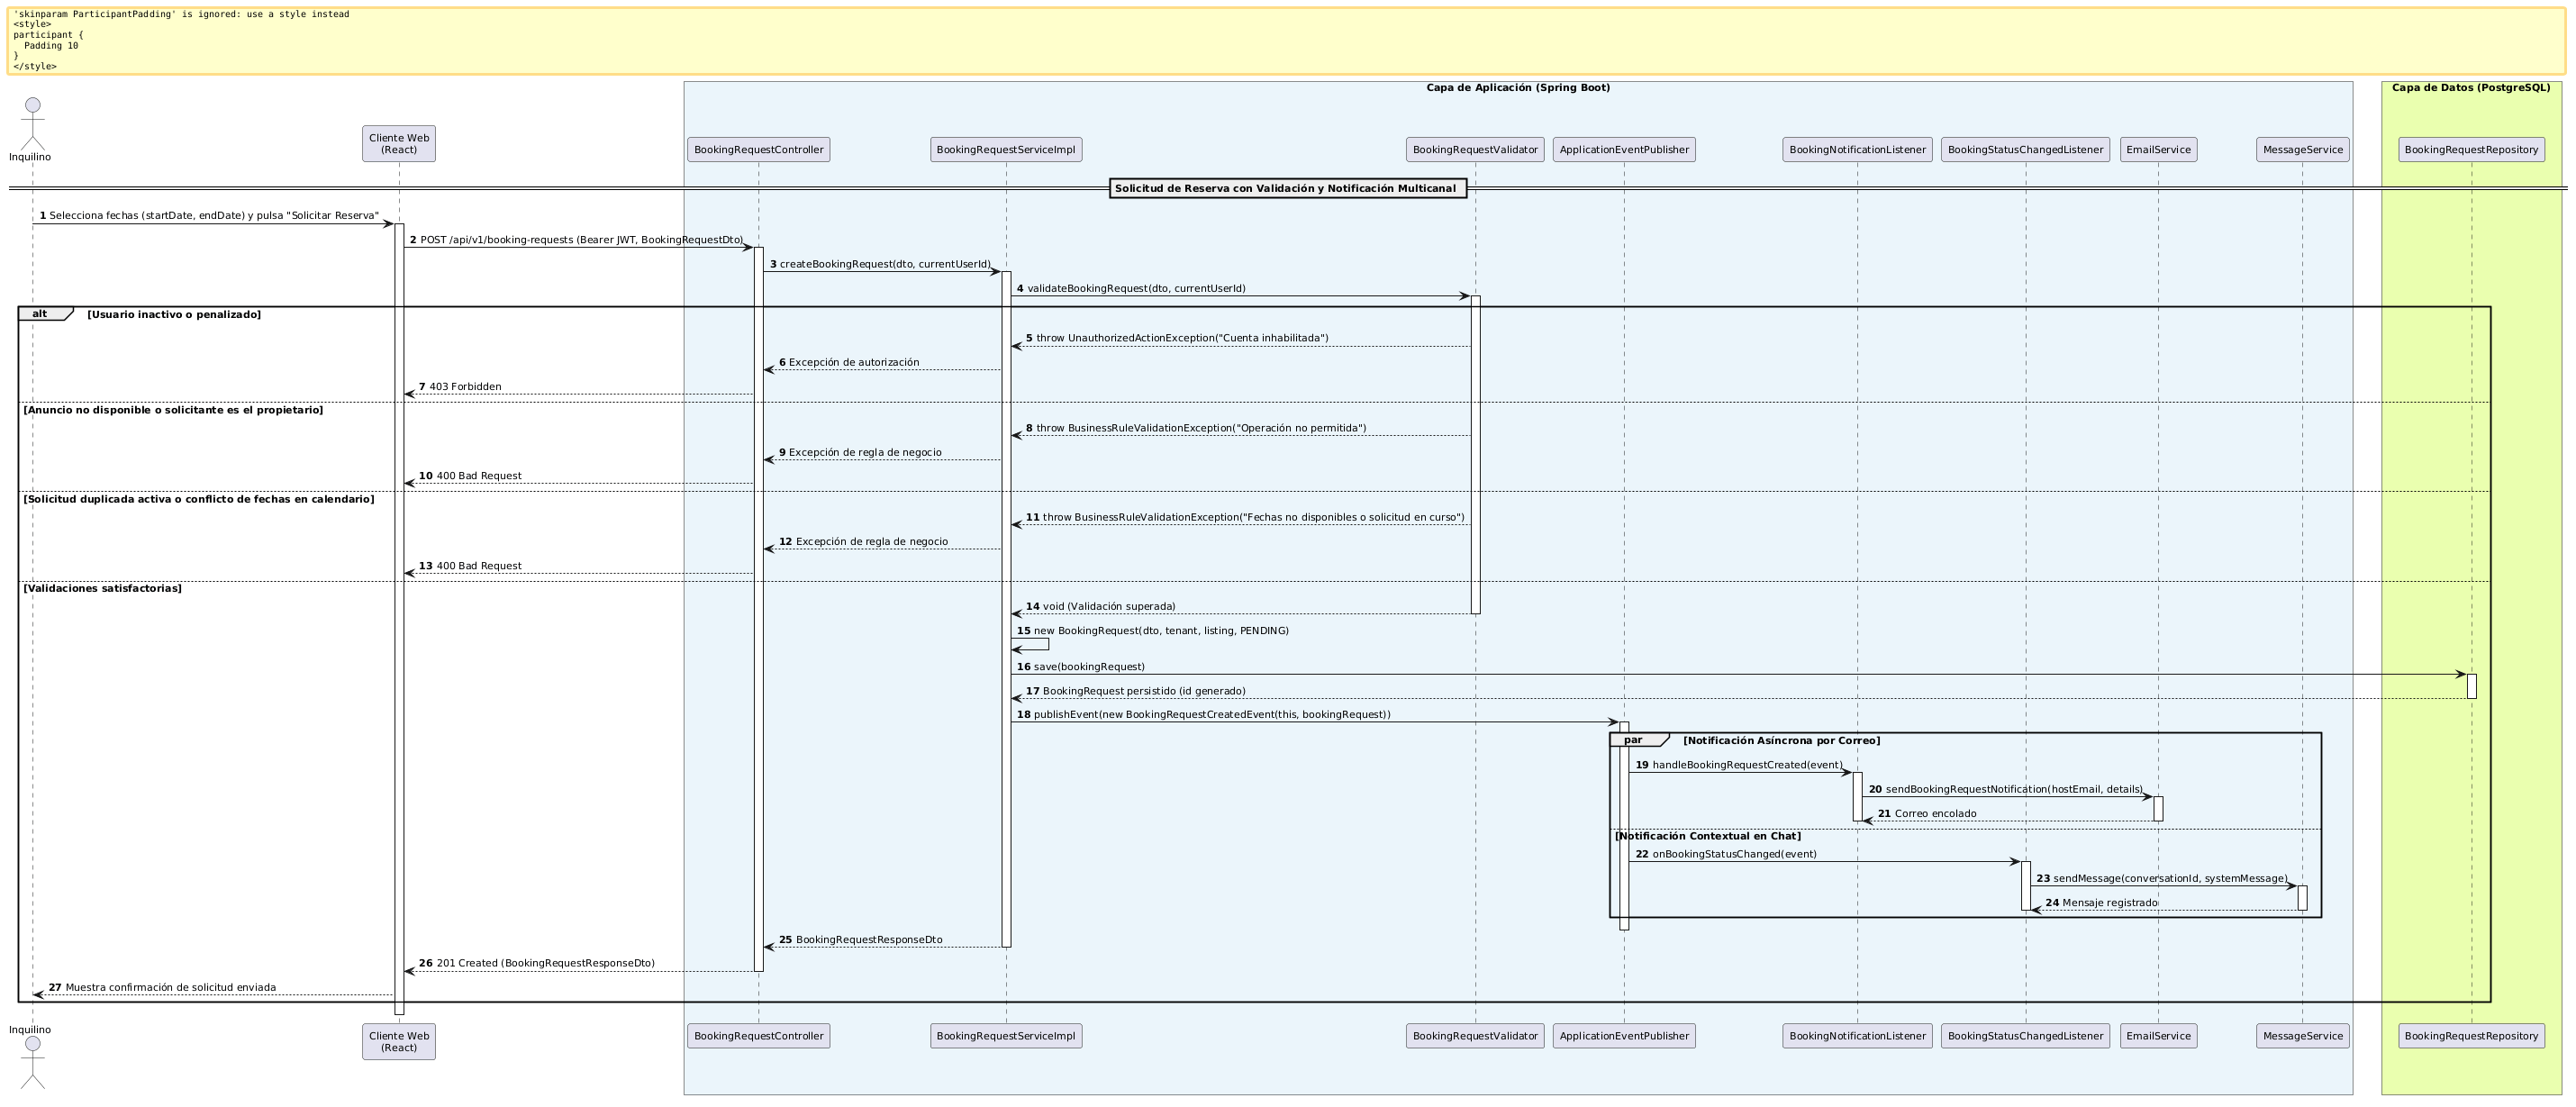
\includegraphics[width=0.95\textwidth]{AnalisisFuncional/img/seq_solicitud_reserva.png}
    \caption{Diagrama de secuencia de la solicitud de reserva con validación temporal y notificación multicanal}
    \label{fig:seq_solicitud_reserva}
\end{figure}

    El inquilino selecciona las fechas en el calendario interactivo y envía la petición mediante \texttt{POST /api/v1/booking-requests}. \texttt{BookingRequestController} recupera la identidad del solicitante desde el token JWT y traslada el objeto \texttt{BookingRequestDto} a \texttt{BookingRequestServiceImpl}. Antes de modificar datos, \texttt{BookingRequestValidator} ejecuta validaciones en cadena: comprueba que el usuario esté activo sin sanciones, que el anuncio permanezca publicado, que el solicitante no sea el dueño del inmueble, que no existan solicitudes duplicadas en trámite y que las fechas no colisionen con reservas confirmadas.

    Tras validar todas las reglas, el servicio instancia la entidad \texttt{BookingRequest} en estado \texttt{PENDING} y la persiste atómicamente en \texttt{BookingRequestRepository}. La transacción publica el evento de dominio \texttt{BookingRequestCreatedEvent} mediante \texttt{ApplicationEventPublisher}. Dos componentes escuchan este evento de forma desacoplada: \texttt{BookingNotificationListener} invoca a \texttt{EmailService} para redactar y enviar un correo transaccional al propietario, mientras \texttt{BookingStatusChangedListener} utiliza \texttt{MessageService} para registrar una notificación automática de sistema dentro de la conversación vinculada al anuncio. El controlador devuelve un código HTTP 201 con el DTO \texttt{BookingRequestResponseDto} confirmando el registro.

    La consolidación de la reserva se produce mediante la aprobación del anfitrión y el pago del depósito de fianza (figura \ref{fig:seq_pago_fianza}).

\begin{figure}[H]
    \centering
    \includegraphics[width=0.95\textwidth]{AnalisisFuncional/img/seq_pago_fianza.png}
    \caption{Diagrama de secuencia de la aceptación de reserva y formalización del cobro de fianza}
    \label{fig:seq_pago_fianza}
\end{figure}

    El anfitrión revisa las solicitudes recibidas y acepta la propuesta llamando a \texttt{PATCH /api/v1/booking-requests/\{id\}/status} con estado \texttt{ACCEPTED}. \texttt{BookingRequestServiceImpl} comprueba que el usuario autenticado sea el titular del inmueble y que la solicitud se encuentre en estado \texttt{PENDING}. Al persistir el cambio, se dispara el evento \texttt{BookingStatusChangedEvent}. El componente \texttt{BookingStatusChangedListener} intercepta el evento e inserta un mensaje de aviso en el chat del inquilino.

    El inquilino abona entonces la fianza mediante \texttt{POST /api/v1/booking-requests/\{id\}/confirm-payment} enviando el DTO \texttt{PaymentConfirmationDto}. El servicio comprueba que quien paga sea el inquilino de la solicitud y que el estado sea \texttt{ACCEPTED}. \texttt{PaymentService} procesa y concilia la transacción económica. Al verificarse el cobro, la entidad \texttt{BookingRequest} guarda los metadatos del pago, conmuta su estado a \texttt{CONFIRMED} y se almacena en base de datos. Se publica el evento \texttt{BookingConfirmedEvent}, permitiendo que \texttt{BookingConfirmedEventListener} bloquee definitivamente el rango de fechas en el calendario del piso frente a peticiones concurrentes.

    La adhesión a una vivienda compartida se gestiona mediante invitaciones temporales de acceso (figura \ref{fig:seq_adhesion_hogar}).

    El compañero de piso introduce el código alfanumérico generado previamente por el administrador del hogar. El servicio comprueba la vigencia temporal del código, verifica que no haya superado su límite de usos y comprueba que el solicitante no pertenezca ya a otra vivienda activa. Tras validar las precondiciones, el backend asocia la cuenta del usuario a la entidad del hogar, asigna el rol de compañero y emite eventos de dominio para actualizar el muro de actividad de los residentes.